\section{openPOWERLINK}
\begin{frame}{openPOWERLINK Stack}
    \begin{itemize}
        \item Open Source implementation of POWERLINK.
        \begin{itemize}
            \item Real-time communication protocol
        \end{itemize}
        \item Distributed under the BSD license, available on GitHub and Sourceforge.
        \item Easy introduction in POWERLINK.
        \item Simple integration of POWERLINK in products.
        \item Improved development influenced by user requests and community contribution.
    \end{itemize}
\end{frame}

\begin{frame}{Structure}
    \begin{columns}
        \begin{column}{0.5\textwidth}
            \begin{block}{Architecture}
                \begin{description}
                    \item[User layer] High level functionalities,API, Asynchronous transmission
                    \item[Kernel layer] Time critical functionalities, synchronization, drivers
                    \item[CAL] Connection between user layer and kernel Layer
                \end{description}
            \end{block}
        \end{column}
        
        \begin{column}{0.5\textwidth}
            \begin{figure}
                \hbox{
                \hspace{-2ex}
                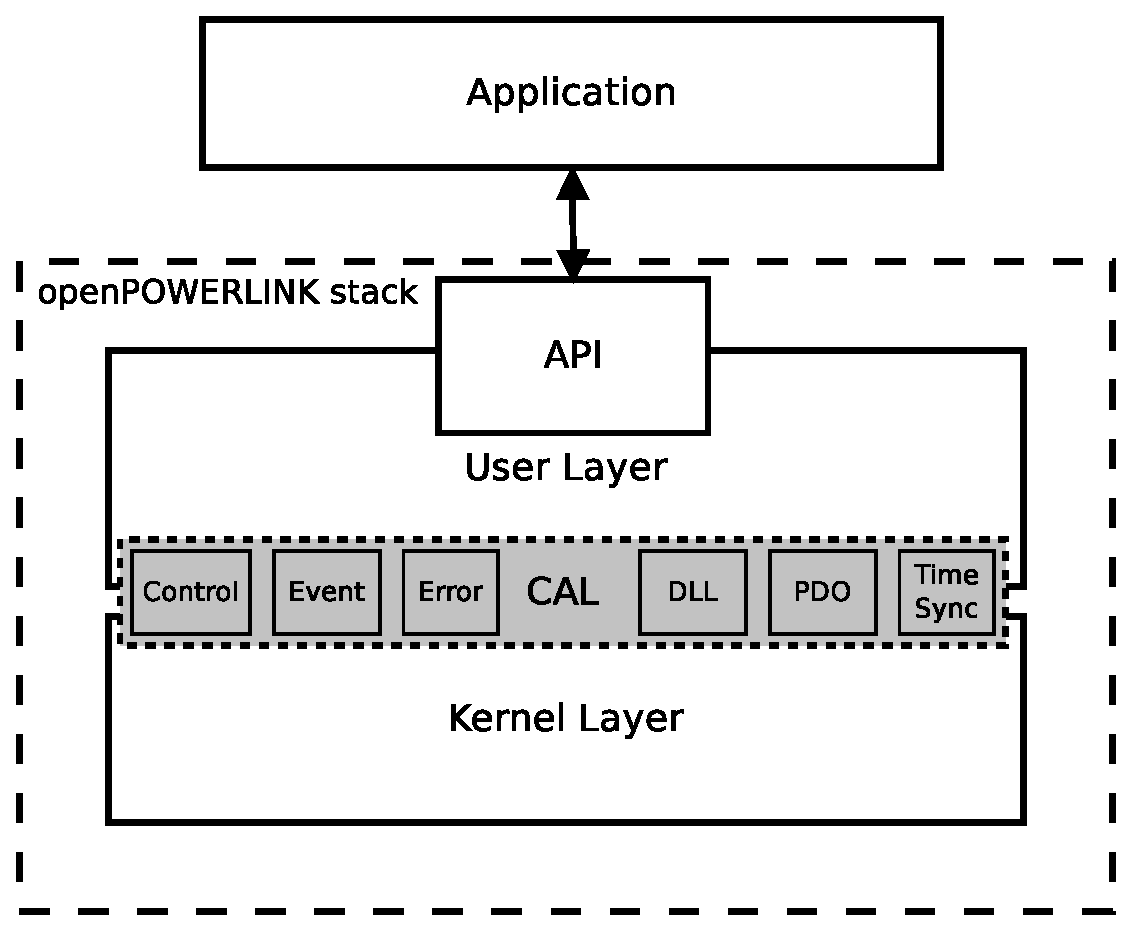
\includegraphics[width=1.2\textwidth]{../../thesis/images/openpowerlink_arch.eps}}
            \end{figure}
        \end{column}
    \end{columns}
\end{frame}

\begin{frame}{Platform Dependency}
    Realized via common header files and platform specific implementations.
    
    \begin{block}{Implemented modules for minimal dependency}
        \begin{description}
            \item[target] General target specific functionalities (Led, IP Address, Default Gateway, Tickcount, sleep)
            \item[edrv] Ethernet driver
            \item[hrestimer] High resolution timer
            \item[sdoudp] Service Data Object (\emph{SDO}) transmission via UDP
            \item[trace] Trace output for debugging
        \end{description}
    \end{block}
\end{frame}

\begin{frame}{Simulation Stub}
    \begin{block}{Target-specific implementation}
        \begin{itemize}
            \item Implementation of all platform dependent modules for \emph{sim} target
            \item Function forwarding to simulation interface
            \item Simple parameter conversions
        \end{itemize}
    \end{block}
    \begin{block}{Simulation interface}
        \begin{itemize}
            \item Separate interface module for each platform dependent module
            \item Store function pointer to external simulation environment
            \item Calling of function pointer with stored instance handle
        \end{itemize}
    \end{block}    
\end{frame}

\begin{frame}{Simulation Stub}
    \begin{figure}
        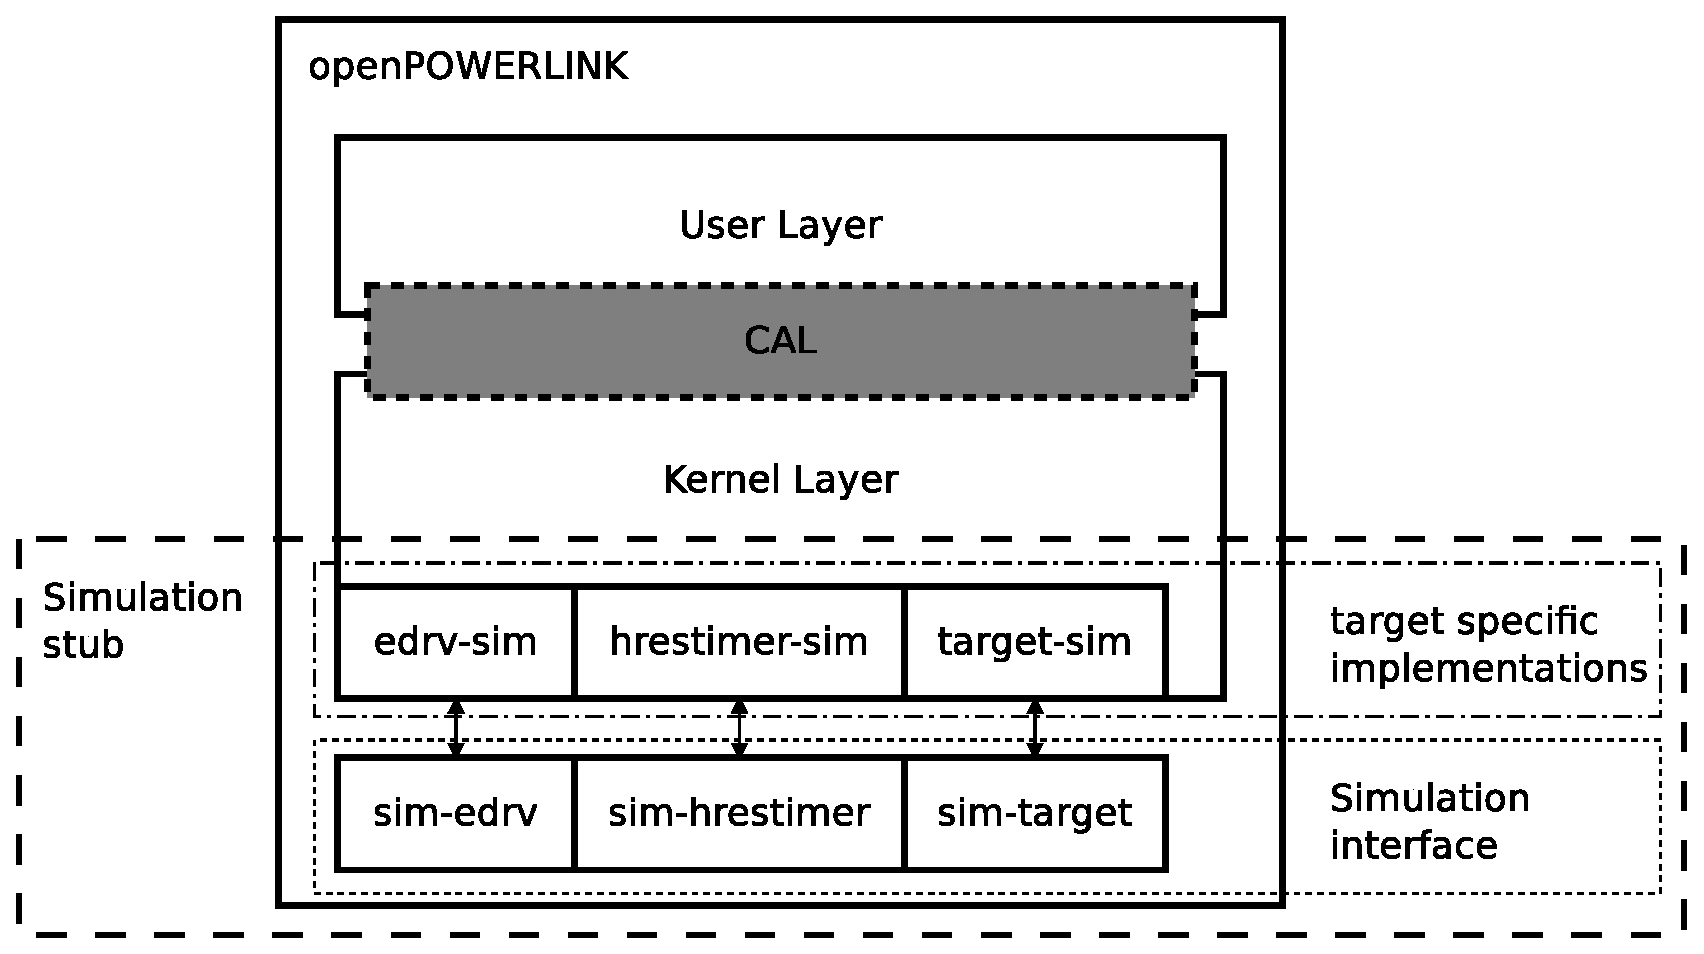
\includegraphics[width=\textwidth]{../../thesis/images/simulation_stub.eps}
    \end{figure}
\end{frame}